\chapter{Módem AM con Etapa de Frecuencia Intermedia}
\label{sec:desarrollo_am}

En este capítulo se presenta el análisis y los resultados de la simulación del módem de Amplitud Modulada (AM)
con portadora y etapa de Frecuencia Intermedia (FI), según lo requerido por la consigna. El circuito guía simulado
en Multisim se muestra en la fig. \ref{crkt.am:circuito}.

\begin{figure}[!ht]
    \centering
    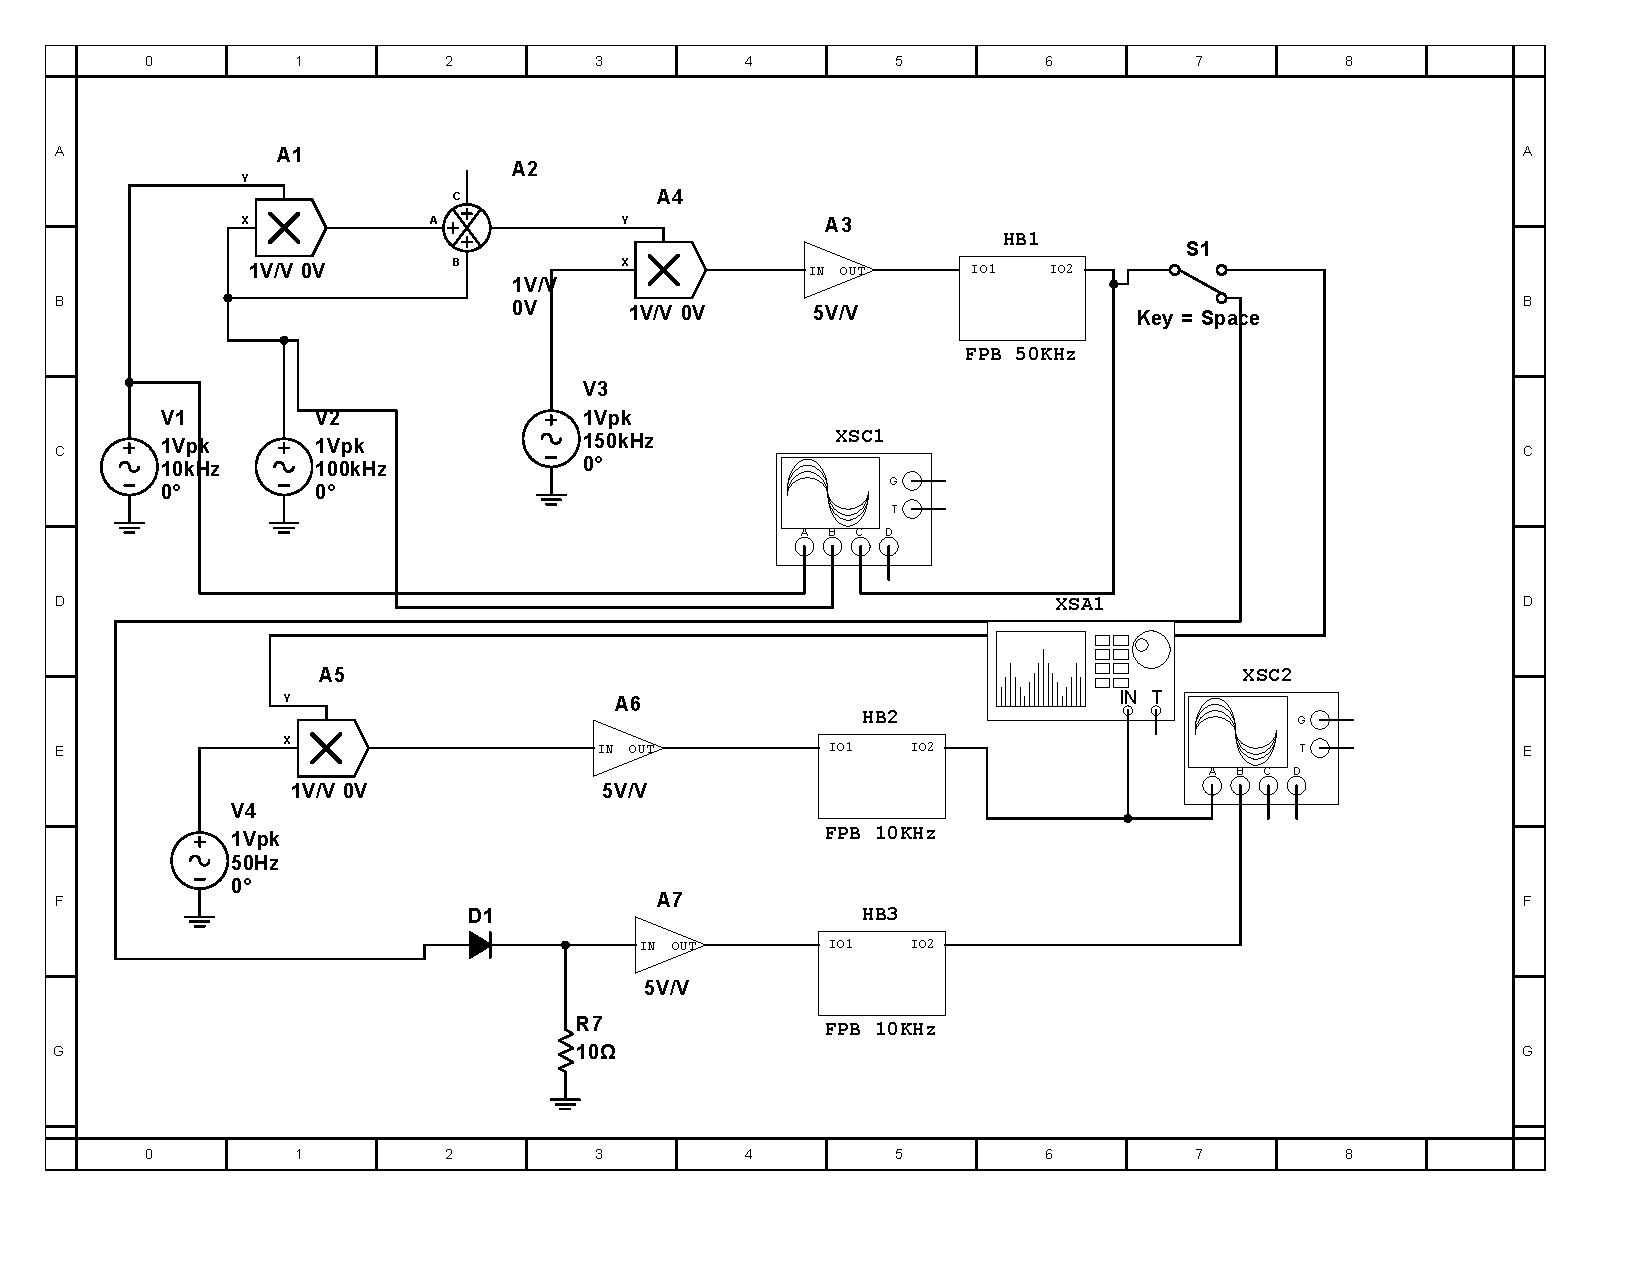
\includegraphics[width=0.95\textwidth]{images/tp1a_circuit.pdf}
    \caption{Circuito del módem AM implementado en Multisim.}
    \label{crkt.am:circuito}
\end{figure}

\section{Modulación de Amplitud (AM)}

La señal de AM con portadora en el dominio del tiempo se describe matemáticamente como:
\begin{equation}
    s_{\text{AM}}(t) = [A_c + m(t)] \cos(2\pi f_c t)
    \label{eq.am:ecuacion_temporal}
\end{equation}
Donde:
\begin{itemize}
    \item $m(t) = A_m \cos(2\pi f_m t)$ es la señal modulante (banda base), con $A_m = 1\V$ y $f_m = 10\kHz$.
    \item $c(t) = A_c \cos(2\pi f_c t)$ es la señal portadora, con $A_c = 1\V$ y $f_c = 100\kHz$.
    \item $m = \frac{A_m}{A_c} = 1$ es el índice de modulación (modulación al $100\%$).
\end{itemize}

Sustituyendo los valores en eq. \ref{eq.am:ecuacion_temporal} y expandiendo trigonométricamente:
\begin{equation}
    s_{\text{AM}}(t) = \cos(2\pi 100\text{k} t) + \frac{1}{2} \cos(2\pi 90\text{k} t) + \frac{1}{2} \cos(2\pi 110\text{k} t)
\end{equation}

El espectro de frecuencia teórico de esta señal consta de tres líneas espectrales:
\begin{itemize}
    \item Portadora en $100\kHz$ con amplitud de $1\V$ ($0\text{ dBV}$).
    \item Banda Lateral Inferior (BLI) en $90\kHz$ con amplitud de $0.5\V$ ($-6\text{ dBV}$).
    \item Banda Lateral Superior (BLS) en $110\kHz$ con amplitud de $0.5\V$ ($-6\text{ dBV}$).
\end{itemize}

\subsection{Punto de Medición A: Señal Modulada en AM}
En el Punto de Medición A se analiza el espectro de la señal de AM obtenida al sumar la portadora al producto de la modulante por la portadora, cuyo resultado se observa en la fig. \ref{fig.am:puntoA_espectro}.

\begin{figure}[!ht]
    \centering
    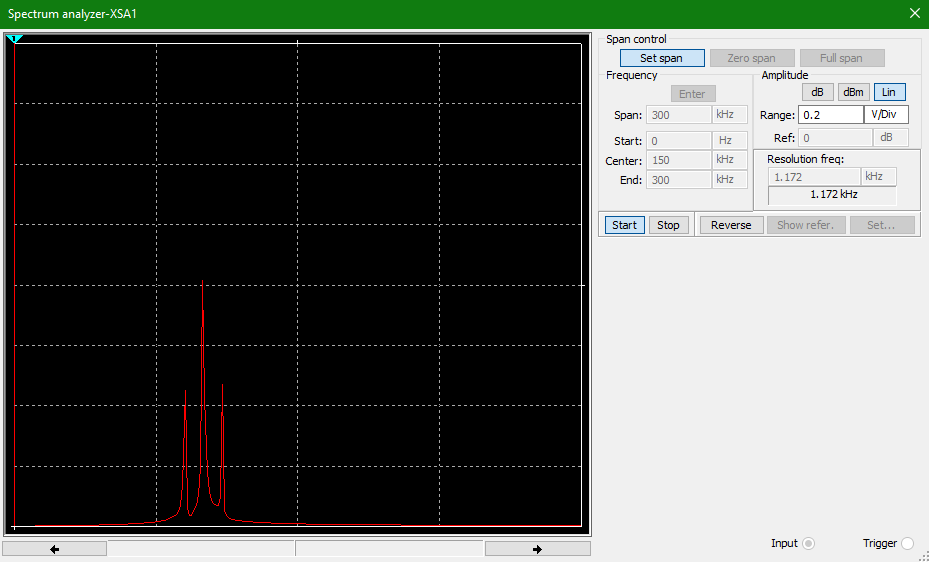
\includegraphics[width=0.75\textwidth]{images/Medicion_A.png}
    \caption{Espectro de frecuencia de la señal AM (Punto A).}
    \label{fig.am:puntoA_espectro}
\end{figure}

\subsection{Modulación AM por Multiplicación Directa (DSB-SC)}
Si se realiza la modulación multiplicando únicamente la señal de banda base con la portadora, se obtiene una señal de
Doble Banda Lateral con Portadora Suprimida (DBL-PS o DSB-SC). La ecuación temporal es:
\begin{equation}
    s_{\text{DSB}}(t) = m(t) \cos(2\pi f_c t) = \cos(2\pi 10\text{k} t)\cos(2\pi 100\text{k} t)
\end{equation}
\begin{equation}
    s_{\text{DSB}}(t) = \frac{1}{2}\cos(2\pi 90\text{k} t) + \frac{1}{2}\cos(2\pi 110\text{k} t)
\end{equation}

El espectro carece de la componente de portadora en $100\kHz$, manteniendo únicamente las dos bandas laterales en
$90\kHz$ y $110\kHz$. Esto mejora la eficiencia energética del transmisor, pero complejiza el receptor ya que
no se puede demodular mediante detección asincrónica por envolvente de forma directa y lineal.

\section{Conversión a Frecuencia Intermedia (FI)}

El proceso de conversión a FI consiste en trasladar el espectro de la señal modulada a una frecuencia central fija
$f_{\text{IF}} = 50\kHz$. Esto se realiza mediante un mezclador (multiplicador) y un oscilador local de frecuencia $f_{\text{LO}}$.

\subsection{Esquema Superheterodino}
En el esquema superheterodino, la frecuencia del oscilador local se sitúa por encima de la portadora:
\begin{equation}
    f_{\text{LO}} = f_c + f_{\text{IF}} = 100\kHz + 50\kHz = 150\kHz
\end{equation}

Al multiplicar $s_{\text{AM}}(t)$ por la señal del oscilador local $\cos(2\pi f_{\text{LO}} t)$, se producen
componentes de suma y diferencia de frecuencias. El espectro de la mezcla en el \textbf{Punto de Medición B} contiene:
\begin{itemize}
    \item Componentes de diferencia (centradas en $f_{\text{IF}} = 50\kHz$): portadora en $50\kHz$, bandas laterales
          en $40\kHz$ y $60\kHz$.
    \item Componentes de suma (centradas en $f_c + f_{\text{LO}} = 250\kHz$): portadora en $250\kHz$, bandas laterales
          en $240\kHz$ y $260\kHz$.
\end{itemize}

\subsection{Esquema Subheterodino}
En el esquema subheterodino, la frecuencia del oscilador local se sitúa por debajo de la portadora:
\begin{equation}
    f_{\text{LO}} = f_c - f_{\text{IF}} = 100\kHz - 50\kHz = 50\kHz
\end{equation}

Al realizar la mezcla, las componentes resultantes son:
\begin{itemize}
    \item Componentes de diferencia (centradas en $f_{\text{IF}} = 50\kHz$): portadora en $50\kHz$, bandas laterales
          en $40\kHz$ y $60\kHz$.
    \item Componentes de suma (centradas en $f_c + f_{\text{LO}} = 150\kHz$): portadora en $150\kHz$, bandas laterales
          en $140\kHz$ y $160\kHz$.
\end{itemize}

\subsection{Comparativa de Mezcla y Filtro de FI (Punto de Medición C)}
Ambos métodos logran trasladar la información a la FI de $50\kHz$. Sin embargo, en el esquema superheterodino las
frecuencias espurias de suma se encuentran mucho más alejadas ($250\kHz$) de la banda de interés ($50\kHz$) en
comparación con el subheterodino ($150\kHz$). Esto facilita el diseño del filtro de FI (pasa-bajos o pasa-banda)
ya que requiere una menor selectividad para atenuar las componentes no deseadas.

En el \textbf{Punto de Medición C}, tras el filtro de FI de $50\kHz$, se obtiene la señal de AM trasladada limpia de
componentes de alta frecuencia.

\begin{figure}[!ht]
    \centering
    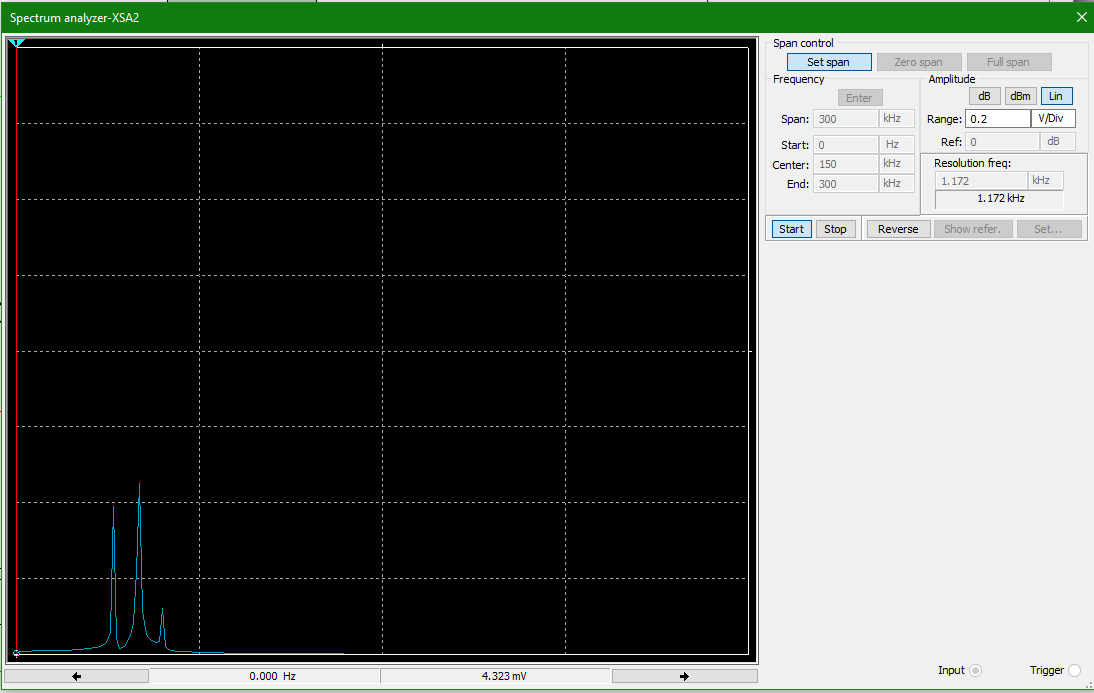
\includegraphics[width=0.75\textwidth]{images/Medicion_B.png}
    \caption{Espectro de frecuencia en la salida del mezclador (Punto B).}
    \label{fig.am:puntoB}
\end{figure}

\begin{figure}[!ht]
    \centering
    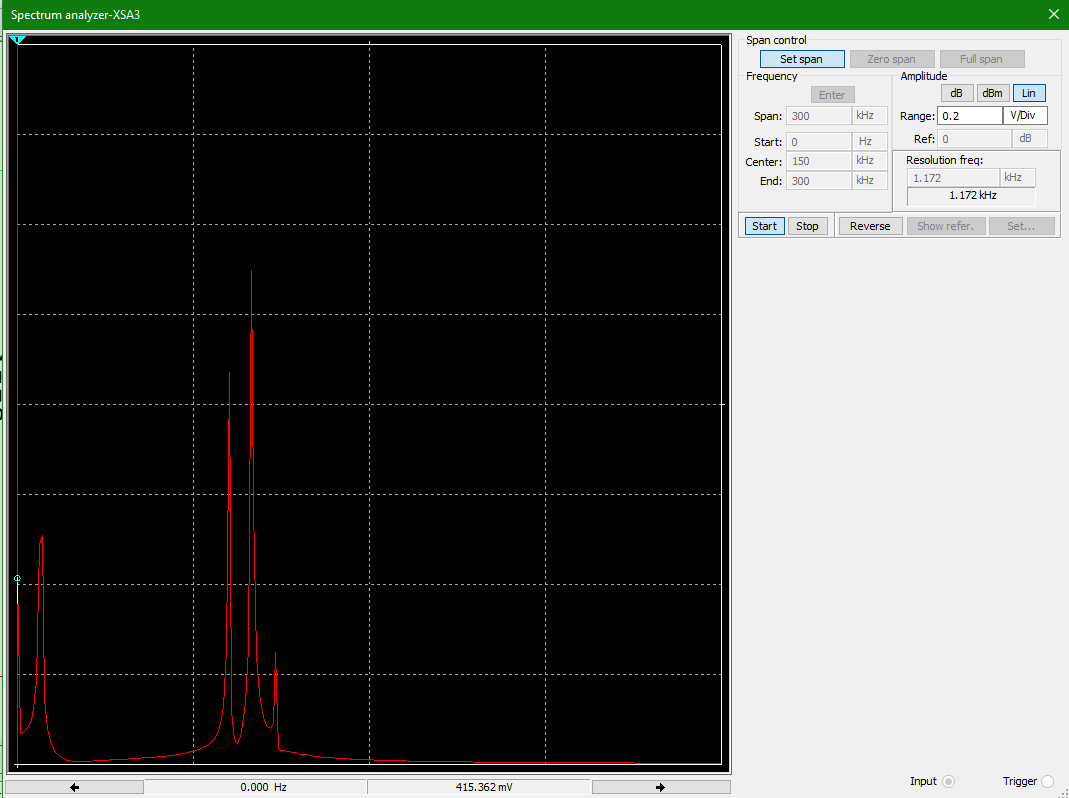
\includegraphics[width=0.75\textwidth]{images/Medicion_C.png}
    \caption{Espectro de la señal filtrada en Frecuencia Intermedia (Punto C).}
    \label{fig.am:puntoC}
\end{figure}

\section{Demodulación de la Señal AM}

Se analizan y simulan los dos métodos de demodulación a partir de la señal de FI:

\subsection{Detección Asincrónica (Detector de Envolvente)}
Se implementa mediante un diodo ideal que rectifica de media onda la señal de FI, seguido de un filtro pasa-bajos
RC (Punto de Medición E).
El diodo elimina los ciclos negativos de la portadora y el filtro suaviza las variaciones rápidas de alta frecuencia.
La constante de tiempo del filtro debe cumplir con la relación de compromiso para evitar el efecto de distorsión
por corte diagonal:
\begin{equation}
    \tau = RC \ll \frac{1}{2\pi f_m}
\end{equation}
Si $RC$ es demasiado grande, el condensador no se descarga lo suficientemente rápido para seguir el decrecimiento de
la modulante. Si es demasiado chico, el rizado de portadora en la salida será muy elevado.

\subsection{Detección Sincrónica}
Se realiza multiplicando la señal de FI por una señal portadora local perfectamente sincronizada en frecuencia
y fase ($50\kHz$). El producto genera componentes en banda base (modulante) y al doble de la frecuencia intermedia
($100\kHz$). Un filtro pasa-bajos posterior elimina la componente de $100\kHz$, recuperando la modulante pura en
el \textbf{Punto de Medición D}.

\begin{figure}[!ht]
    \centering
    \begin{subfigure}[b]{0.48\textwidth}
        \centering
        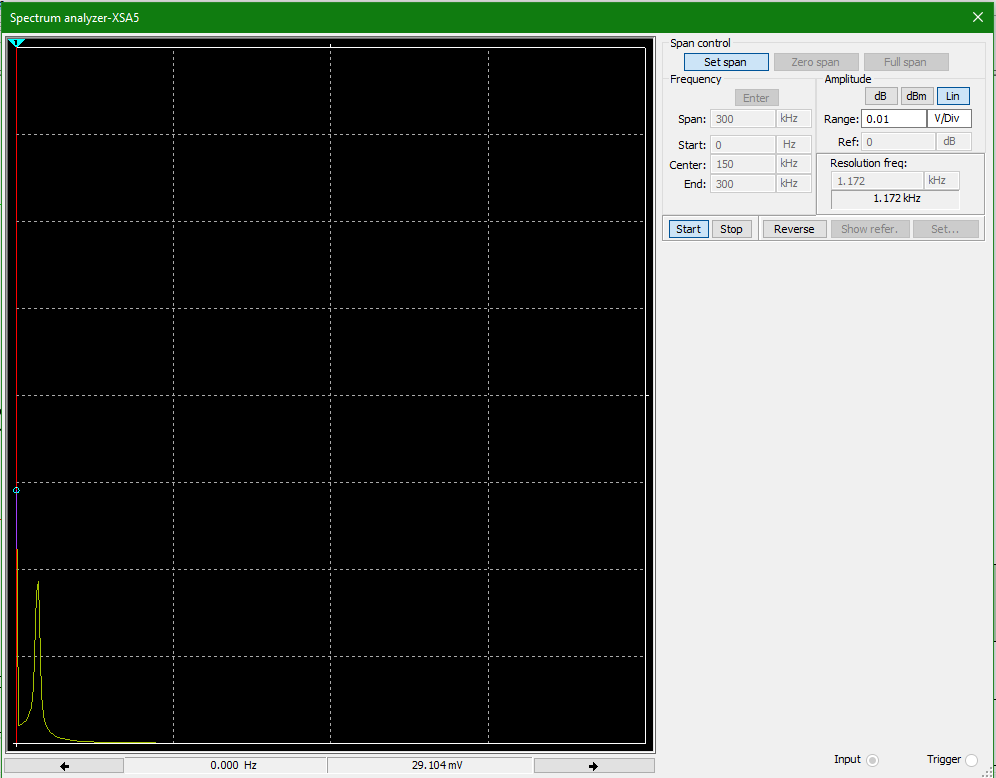
\includegraphics[width=\textwidth]{images/Medicion_E_Sincronica.png}
        \caption{Detección sincrónica (Punto D).}
        \label{fig.am:demodulacion_sincronica}
    \end{subfigure}
    \hfill
    \begin{subfigure}[b]{0.48\textwidth}
        \centering
        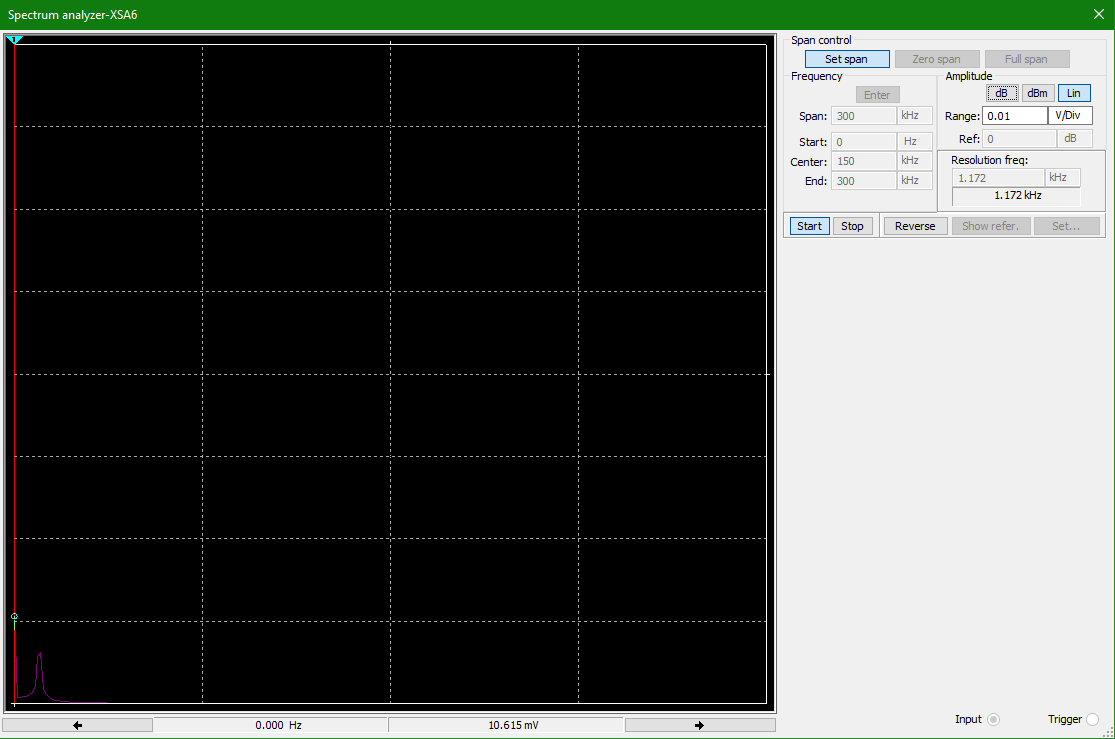
\includegraphics[width=\textwidth]{images/Medicion_E_asincronica.png}
        \caption{Detección asincrónica (Punto E).}
        \label{fig.am:demodulacion_asincronica}
    \end{subfigure}
    \caption{Espectro de las señales demoduladas por detección sincrónica (Punto D) y asincrónica (Punto E).}
    \label{fig.am:demodulacion}
\end{figure}

\subsection{Comparación entre Detecciones}
\begin{table}[!ht]
    \centering
    \caption{Comparativa entre Detección Sincrónica y Asincrónica en AM.}
    \label{tab.am:comparacion}
    \begin{tabular}{|l|p{5cm}|p{5cm}|}
        \hline
        \textbf{Característica} & \textbf{Detección Asincrónica} & \textbf{Detección Sincrónica} \\ \hline
        \textbf{Complejidad} & Muy baja (Diodo y filtro RC). & Alta (Requiere oscilador local y sincronía). \\ \hline
        \textbf{Linealidad} & Sufre distorsión con $m > 1$ o con portadora suprimida. & Lineal para cualquier $m$ y para portadora suprimida. \\ \hline
        \textbf{Ruido} & Mayor susceptibilidad al ruido. & Mejor relación señal-ruido. \\ \hline
        \textbf{Distorsión} & Rizado residual y riesgo de corte diagonal. & Prácticamente libre de distorsión de fase/amplitud. \\ \hline
    \end{tabular}
\end{table}
